\section{Motivation} \label{sec:motivation}
Nowadays, the main stream training frameworks typically adopt the offline training
on GPPs to obtain the neural network models and then apply the quantized models to the 
target CNN accelerators. When the computing on the underlying CNN accelerators differs
from that calculated with GPPs due to the approximate arithmetic logic, overclocking or 
soft errors, the offline trained neural network models executed on the accelerator 
may deviate from the expected computing result. To evaluate the influence, 
we take Alexnet as an example to evaluate the prediction 
accuracy loss when the offline trained model is deployed on the CNN 
accelerators with approximate multiplier, overclocking, and soft errors respectively. 

In the experiment, we use PipeCNN\cite{pipecnn_2}, an open sourced high-level CNN accelerator, 
as the baseline design. We have it implemented on KCU1500 FPGA board and run at 210 MHz. 
On ImageNet, we train AlexNet offline and then apply it to the 8-bit accelerator. 
The resulting top-1 accuracy and top-5 accuracy of Alexnet on the accelerator 
is 54.2\% and 78.06\% respectively. On top of the baseline accelerator, we apply 
approximate multiplier, overclocking and soft error injection respectively. 

In the approximate computing case, we implement the dynamic-range approximate 
multiplier proposed in \cite{Approximate_Multiplier_31}. Basically, the multiplier 
will keep the non-zero most significant bit as well as the following $k$ bits in the 
multiplication to simplify the hardware design and improve the energy efficiency.
In this experiment, we set $k$ to be 2. In the overclocking case, we boost the clock frequency 
to the extreme clock and the design achieves 260 MHz in the experiment. 
In the soft error scenario, we inject SEU errors with a uniform distribution model to 
both the on-chip buffers and the arithmetic units. The injection rate is set to be 
1E-7 which means one random bit flops every 1E7 operations. Note that the soft error is modeled 
on top of the PipeCNN C model instead of the real hardware.

With the conventional offline training approach, the offline trained Alexnet model 
will be deployed directly. The model accuracy loss on ImageNet in the three scenarios is 
measured and presented in Figure \ref{fig:loss}. Top-1 prediction accuracy loss 
typically is more than 10\% in all the three cases while top-5 accuracy loss is slightly 
lower. Particularly, we want to emphasize that the prediction accuracy loss is extremely large 
from the perspective of neural network models, because the prediction accuracy gap of 
large models and small models is only a few percent according to the statistic in \cite{model-accuracy}.

\begin{figure}
	\center{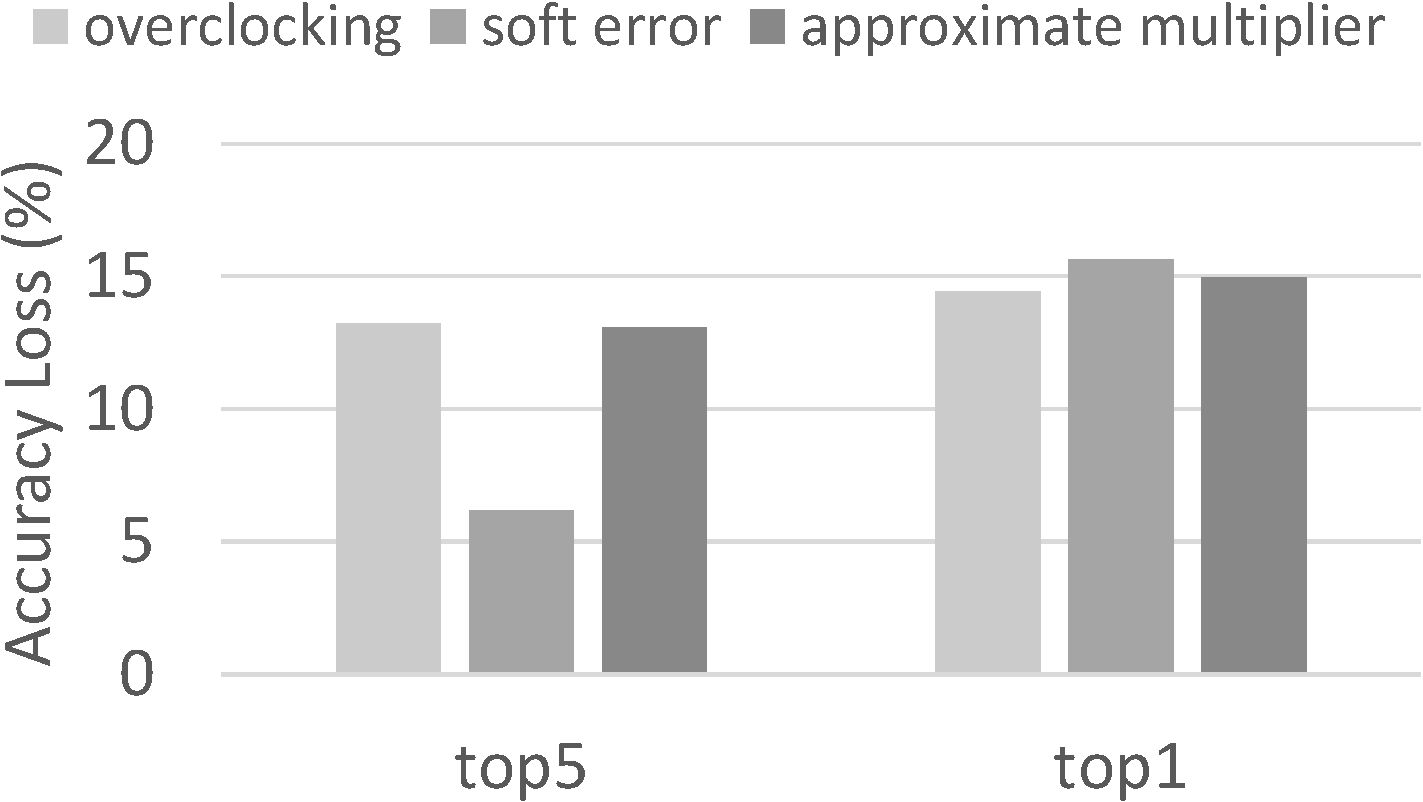
\includegraphics[width=0.75\linewidth]{Loss}}
    \caption{Prediction accuracy loss of the offline trained Alexnet on CNN accelerators with approximate multiplier, overclocking and soft errors.}
\label{fig:loss}
\vspace{-1em}
\end{figure}


